\subsubsection{Graphs \& Trees}

\textbf{To add a node:}
\begin{figure}[H]
    \centering
    \setlength{\fboxsep}{0pt}
    \setlength{\fboxrule}{1pt}
    \fbox{
        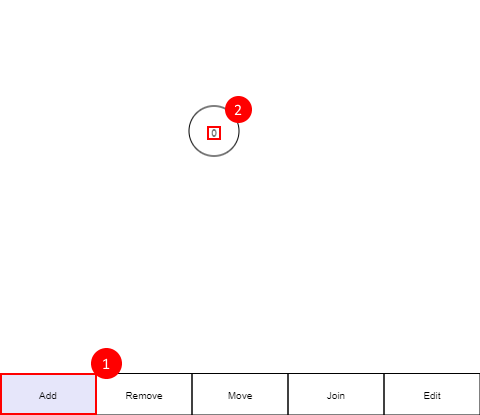
\includegraphics[width=0.65\linewidth]{/userManual/graphdrawer/addnode}
    }
    \caption{}
    \label{fig:addNode}	
\end{figure}
\begin{userManualItemlist}
    \item[Step I.] Click the "Add" button (1). (Figure: \ref{fig:addNode})
    \item[Step II.] Click the position where you want the node to be (2). (Figure: \ref{fig:addNode}) 
\end{userManualItemlist}

\textbf{To remove a node:}
\begin{userManualItemlist}
    \item[Step I.] Click the "Remove" button.
    \item[Step II.] Click the node.
\end{userManualItemlist}

\textbf{To move a node:}
\begin{userManualItemlist}
    \item[Step I.] Click the "Move" button.
    \item[Step II.] Press the mouse button while the cursor is inside the node.
    \item[Step III.] Move the cursor to the new position.
    \item[Step IV.] Release the mouse button.
\end{userManualItemlist}

\textbf{To join two nodes:}
\begin{userManualItemlist}
    \item[Step I.] Click the "Join" button.
    \item[Step II.] Press the mouse button while the cursor is inside the first node.
    \item[Step III.] Move the cursor inside the other node.
    \item[Step IV.] Release the mouse button. 
\end{userManualItemlist}

\textbf{To edit the value of a node:}
\begin{userManualItemlist}
    \item[Step I.] Click the "Join" button.
    \item[Step II.] Click the node.
    \item[Step III.] Type the new value in the prompt.
    \item[Step IV.] Click the "OK" button. 
\end{userManualItemlist}